%% ===========================================================================
%%  Regime-Aware Temporal Granularity for Causal Video World Models
%%  Target: Computer Vision and Image Understanding (Elsevier), CAS single column
%%  Compile: pdflatex -> bibtex -> pdflatex x2
%% ===========================================================================
\documentclass[review]{cas-sc}          % single column; 'review' adds line numbers
\usepackage[numbers,sort&compress]{natbib}
\usepackage{amsmath,amssymb}
\usepackage{graphicx}
\usepackage{booktabs}
\usepackage{multirow}
\usepackage{xcolor}

\shorttitle{Regime-Aware Temporal Granularity}
\shortauthors{H. M. Jisan}

\begin{document}

\title[mode=title]{Regime-Aware Temporal Granularity for Causal Video World Models:\\
When Does Adaptivity Pay?}

\author[1]{Hossen Md Jisan}[orcid=0009-0004-9571-1450]
\affiliation[1]{organization={Department of Artificial Intelligence, Nanjing University of
Information Science and Technology (NUIST)}, city={Nanjing}, country={China}}
\cortext[1]{Corresponding author.}
\ead{jisanahammed1952@gmail.com}

\begin{abstract}
Causal video generators produce a rollout one temporal chunk at a time, so spending expensive per-frame
compute only on hard segments looks attractive. We show that this idea rests on three
\emph{preconditions} --- cost, signal and endpoint --- and that all three are \emph{regime properties}
rather than universal facts. On a matched two-GPU study (Tesla T4 and A100-80GB) of a causal diffusion
backbone, we (i) measure the per-forward cost against the schedule break-even and find the same mode pair
on opposite sides of the inequality; (ii) show that cheap context statistics cannot predict coarse-unsafe
segments (AUROC 0.491), while an \emph{intrinsic} probe computed from the generator's own prefill
activations reaches 0.798 and, combined with a sampler convergence residual, 0.842; and (iii) demonstrate
that an endpoint independent of the compared modes is mandatory, because the internal reference reverses
between GPUs. We then derive a \emph{regime map} that states exactly when adaptivity pays: only when the
cheap mode is cheaper \emph{and} worse. Across two GPUs and three independent endpoints (latent,
decoded-pixel, temporal flicker) our operating points fall outside that region --- the cheap mode was
never worse --- so the optimal policy is a \emph{fixed} mode, and a router is unnecessary. We also report
a training-free seam repair that reduces the switch-boundary discontinuity by 25\% while improving
fidelity, quantify drift propagation, and record three boundaries: signals do not transfer across GPUs
(the intrinsic probe inverts, 0.798~$\rightarrow$~0.143), drift is linear and policy-insensitive, and a
context-free decision-model critic is at chance. All results, figures and audited result files are public.
\end{abstract}

\begin{keywords}
causal video generation \sep video world models \sep autoregressive diffusion \sep adaptive compute \sep
temporal granularity \sep regime map \sep efficient inference
\end{keywords}

\maketitle

%% ===========================================================================
\section{Introduction}
\label{sec:intro}

Interactive video world models --- game engines, robot simulators, embodied agents and augmented
reality --- must synthesise frames under a latency budget on whatever accelerator is available. A causal
(autoregressive) video generator emits the rollout one temporal chunk at a time, and chunks are not
equally hard. It is therefore natural to spend \emph{fine} per-frame computation on difficult segments
and a cheaper \emph{coarse} multi-frame mode elsewhere, deciding before each segment is generated.

This idea is appealing but conditional. Our earlier study~\citep{hossen2026jevRouted} framed it as
resting on three \emph{preconditions}: (P1) a cheap mode must be genuinely cheaper on the deployment
hardware at the chosen schedule; (P2) a signal available \emph{before} generation must predict which
segments are unsafe for the cheap mode; and (P3) the quality claim must be certified by an endpoint that
is independent of the modes being compared. That study measured the preconditions on a single GPU and
reported a conditional trade-off.

This paper asks the question that follows: \emph{when does adaptivity actually pay?} We answer with a
matched two-GPU study (Tesla T4 and A100-80GB) of a causal diffusion backbone, and we make four
contributions.

\begin{itemize}
  \item \textbf{A two-GPU regime map} (\S\ref{sec:method}) that partitions the
  (cost-ratio, quality-gap) plane into three policies --- fixed fine, fixed coarse and adaptive --- and
  states precisely when a router is worth deploying. The adaptive region is defined by a conjunction:
  the cheap mode must be \emph{cheaper} \emph{and} \emph{worse}.
  \item \textbf{An intrinsic signal.} A probe on the generator's own prefill activations predicts
  coarse-unsafe segments at AUROC 0.798 with no external oracle, against 0.491 for hand-crafted context
  statistics. A sampler \emph{convergence residual} --- the ratio of the last to the first denoising-step
  update magnitude --- adds independent information, and the two together reach 0.842.
  \item \textbf{A training-free seam repair.} Switching modes creates a measurable discontinuity at the
  boundary. Blending the first latent frame of the new segment toward the boundary by 25\% reduces the
  seam by 25\% \emph{and} improves fidelity, with no training.
  \item \textbf{A boundary analysis.} We show, and record, that signals are regime properties: the
  intrinsic probe \emph{inverts} on the second GPU (0.798~$\rightarrow$~0.143). Drift is linear and not
  predictable from the policy, and a decision-model critic shown only pixels is at chance. Each boundary
  is stated with the experiment that produced it.
\end{itemize}

A summary of the programme is shown in Fig.~\ref{fig:arch}. Throughout, we report the \emph{measured}
limit of each naive formulation rather than treating it as a failure; the boundaries are the paper's
design output.

\begin{figure*}[t]
  \centering
  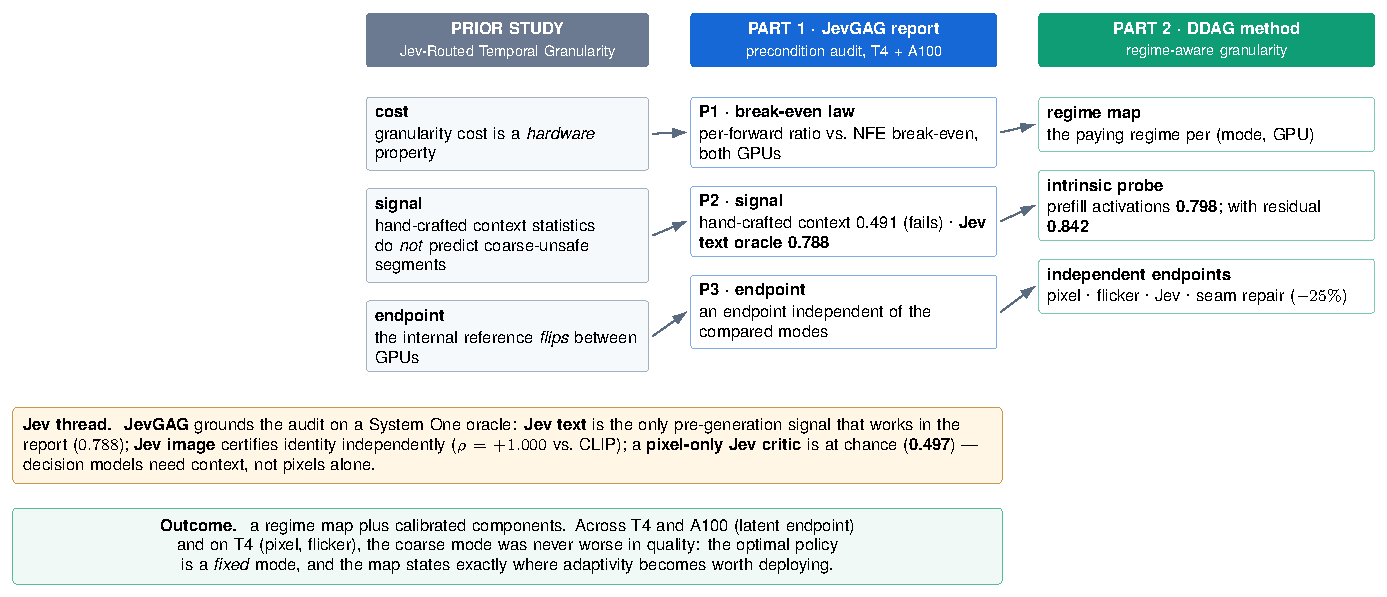
\includegraphics[width=\textwidth]{figures/fig_architecture.pdf}
  \caption{The programme. The earlier study established three preconditions; the report in this work
  measures them on two GPUs; the method turns them into a regime map and calibrated components. Each row
  is one precondition --- the boundary found and its resolution. The decision-model (Jev) thread that
  grounds the audit is highlighted.}
  \label{fig:arch}
\end{figure*}

%% ===========================================================================
\section{Related Work}
\label{sec:related}

\paragraph{Causal and autoregressive video generation.}
Streaming video generators produce a rollout chunk by chunk, and the train--test gap between teacher
forcing and self-rolling is a central difficulty~\citep{huang2025self,zhu2026causal,zhao2026causal}.
Recent recipes distil few-step causal diffusion models for interactive use~\citep{zheng2026causalrcm,zhao2026minwm},
and autoregressive transformer generators scale similar ideas~\citep{ai2025magi1}. Our backbone is a
causal distilled diffusion model of this family; we treat it as a black box and study its
\emph{granularity}, not its training.

\paragraph{Adaptive compute and routing.}
Adaptive computation was introduced for recurrent networks~\citep{graves2016adaptive} and early exiting for
classification~\citep{teerapittayanon2017branchynet,wang2017skipnet}. In generative video, recent work
allocates computation by step or by token: dynamic step allocation~\citep{le2026dsa}, learned flexible
chunking~\citep{ma2026flexforcing}, pruning and routing~\citep{wang2026pare}, layer reuse~\citep{adnan2025foresight},
and caching of attention or flow state~\citep{ma2026flow,xu2026motionaware,wang2026inflight,song2026trac}.
Adaptive tokenisation changes the \emph{representation}~\citep{li2025learning,xiong2026evatok,yuan2025dlfrvae,zhong2025vfrtok}.
Our work differs in object and in method: we route the \emph{temporal granularity} of a fixed backbone,
and --- crucially --- we do not assume that routing pays; we characterise the regime in which it does.

\paragraph{Internal probes and verification.}
Ensembles of internal classifiers and early-exit policies read a network's own intermediate
representations~\citep{sun2021early,xu2023lgvit,yoo2026adept,zeng2023consistentee,zhou2020bert}. We adapt this
idea to \emph{generation-mode safety}: a probe on a diffusion transformer's prefill activations predicts
whether a cheap mode is unsafe for the upcoming segment. Verification-first policies are related to
speculative decoding~\citep{chen2026dflash,liu2024pearl,li2026is}, but speculation there
operates over tokens; here it operates over the temporal-chunking axis.

\paragraph{Evaluation of generative video.}
Video generative models are evaluated along many axes, including temporal
flickering~\citep{huang2024vbench,zheng2025vbench20}, artefact taxonomies~\citep{zhu2026artifactaware}, and
compression-aware consistency~\citep{zsoldos2026evaluating}. We adopt a multi-endpoint protocol: a latent
reference, a decoded-pixel reference and a temporal-flicker statistic, so that a claim cannot be an
artefact of one metric.

\paragraph{Decision models.}
System One decision models return typed, calibrated answers rather than generated
text~\citep{ling2026jev,geuter2026releasing,li2026llmasjev}. Our earlier study used such a model
as an off-device routing oracle; here we test it as a \emph{critic} and report the boundary we find,
consistent with independent evidence that pixel-only quality prediction with such models is
unreliable~\citep{robitza2026jevqa}.

%% ===========================================================================
\section{Background: the three preconditions}
\label{sec:background}

\paragraph{Setting.}
A causal generator with two granularity modes is rolled out over $T$ segments. A \emph{fine} mode emits
one latent frame per chunk; a \emph{coarse} mode emits $K$ frames jointly. A policy chooses a mode per
segment. We write $c_f, c_c$ for the per-segment cost of the two modes and $q_f, q_c$ for a quality
functional (lower is better).

\paragraph{The three preconditions.}
\begin{description}
  \item[P1 (cost).] The cheap mode must satisfy $c_c < c_f$ on the deployment hardware at the chosen
  schedule. Because a coarse forward is heavier than a fine forward, the condition is a comparison of the
  measured per-forward ratio against the \emph{break-even} set by the number of function evaluations of
  each schedule, $\rho_\text{be} = \mathrm{NFE}_f / \mathrm{NFE}_c$.
  \item[P2 (signal).] A quantity computable \emph{before} a segment is generated must separate segments
  for which the cheap mode is unsafe. The earlier study found that hand-crafted context statistics fail
  this test and that an off-device decision model passes it.
  \item[P3 (endpoint).] The quality claim must be certified by a measure that is independent of the two
  modes. The earlier study found that an internal reference reverses direction between GPUs.
\end{description}

\paragraph{Matched design and label.}
For every prompt and segment we generate \emph{both} modes from the same boundary and the same noise, so
that the only difference is the generator. A segment is \emph{coarse-unsafe} when the coarse segment is
farther from a high-quality reference than the fine segment. Unless stated otherwise the reference is a
four-step fine rollout, and the label is
$y = \mathbb{1}[\,\ell(q_c) > \ell(q_f)\,]$ with $\ell$ the endpoint distance.

\paragraph{The report.}
On T4 the report finds that coarse is \emph{not} cheaper for a two-step coarse schedule, that hand-crafted
context statistics reach only 0.491 AUROC while a decision-model text oracle reaches 0.788, and that the
internal reference flips between GPUs. On A100 the cost ordering reverses. The report also shows that a
two-threshold controller with a hysteresis band and a forced-recovery window stabilises switching, and
that switching leaves a measurable \emph{seam}. Full details, code and audited result files are in the
repository accompanying this paper.

%% ===========================================================================
\section{Method: regime-aware granularity}
\label{sec:method}

\subsection{The regime map}
\label{sec:regimemap}

Let $r = c_c / c_f$ be the cost ratio and $\Delta = q_c - q_f$ the quality gap, with $\Delta > 0$ meaning
the cheap mode is worse. The plane is partitioned into three policies:
\begin{equation}
\text{policy} =
\begin{cases}
\text{fixed fine}, & r > 1 \quad \text{(the cheap mode is dearer)},\\
\text{adaptive},   & r < 1 \ \wedge\ \Delta > 0 \quad \text{(cheaper and worse)},\\
\text{fixed coarse}, & r < 1 \ \wedge\ \Delta \le 0 \quad \text{(cheaper and no worse)}.
\end{cases}
\label{eq:regime}
\end{equation}
Equation~\eqref{eq:regime} is the method's core: a router is worth deploying \emph{only} in the middle
region. Outside it, one mode dominates and the routing machinery is pure overhead. Figure~\ref{fig:regime}
plots our operating points in this plane.

\begin{figure}[t]
  \centering
  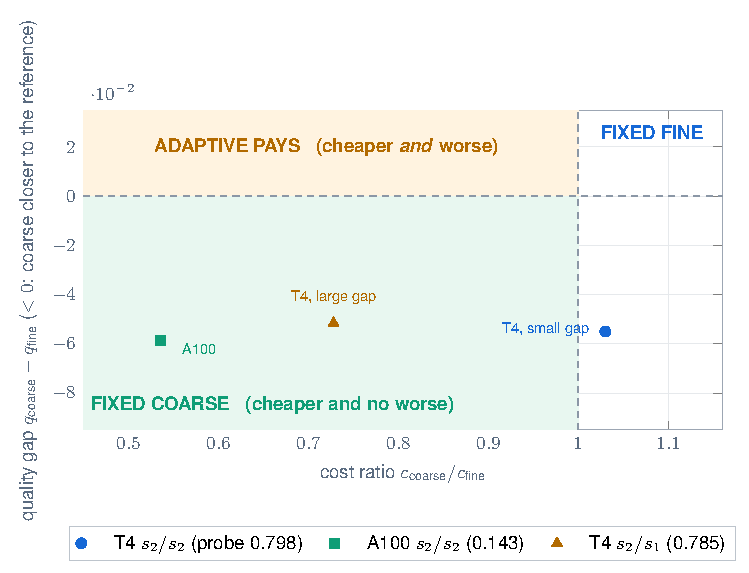
\includegraphics[width=\columnwidth]{figures/fig_regime_map.pdf}
  \caption{The regime map. The adaptive region (upper left, shaded) is empty at every operating point we
  measured: across both GPUs the cheap mode was never worse, so the optimal policy is a fixed mode.
  Markers are labelled with the schedule pair and the intrinsic-probe AUROC at that point.}
  \label{fig:regime}
\end{figure}

\subsection{An intrinsic pre-generation probe}
\label{sec:probe}

At the decision point for a segment, the generator has already encoded the boundary context. We capture
the pooled output of each transformer block of the single prefill forward on the boundary and fit a
logistic probe on a chosen block. The probe is a \emph{pre-generation} quantity: it uses only activations
the rollout has already computed, requires no external service, and adds no measurable latency. The probe
is evaluated with leave-one-prompt-out cross-validation, so no segment is scored by a model that has seen
its own prompt.

\subsection{A convergence residual}
\label{sec:crv}

A distilled few-step sampler has no explicit error estimate, but its update magnitudes are observable.
Let $v_1, \dots, v_S$ be the norm of the predicted velocity at each denoising step of a segment. We define
the \emph{convergence residual}
\begin{equation}
\kappa = v_S / v_1 ,
\label{eq:kappa}
\end{equation}
the ratio of the last to the first step magnitude. A sampler that has settled produces $\kappa \ll 1$; a
sampler still moving at its final step produces $\kappa \approx 1$. Because $\kappa$ is computed from
quantities the sampler already produces, it is free. We report the \emph{direct} AUROC of $\kappa$; a
logistic model trained on a single scalar would re-learn its sign and mask an inverted signal.

\subsection{Calibrated gating}
\label{sec:gate}

Given a score $u$ that increases with expected unsafety, a gate escalates a segment to the fine mode when
$u > \tau$. Two regimes are distinguished. In \emph{routing} the gate chooses the mode before generation;
in \emph{escalation} the cheap mode is always generated and the fine mode is recomputed when the gate
fires. With escalation rate $\rho$, escalation costs $c_c + \rho\,c_f$ against $c_f$ for fixed fine, so a
saving requires $\rho < 1 - r$; routing costs $(1-\rho)c_c + \rho c_f$ and saves whenever $r < 1$. This
is why the cost precondition, not the signal, is the binding constraint.

\subsection{Training-free seam repair}
\label{sec:seam}

When the mode changes at a boundary, the first frame of the new segment is generated by a different
generator than the frame before it, and the adjacent-frame distance at that boundary exceeds the
interior. We repair it without training: the first latent frame of the incoming segment is blended toward
the boundary frame,
\begin{equation}
\tilde{x}_1 = (1-\alpha)\,x_1 + \alpha\,b ,
\label{eq:blend}
\end{equation}
with $b$ the boundary latent and $\alpha$ a scalar. We sweep $\alpha$ and report the seam--fidelity
frontier.

%% ===========================================================================
\section{Experimental protocol}
\label{sec:protocol}

\paragraph{Backbone and hardware.}
A causal distilled diffusion video model (1.3B) at $480\times832$; a four-step fine rollout is the
reference. Two accelerators: a \textbf{Tesla T4} (Turing, SDPA attention) and an
\textbf{A100-80GB} (Ampere, FlashAttention-2). The same prompts, seed, horizon and code are used on both.

\paragraph{Prompts and horizon.}
Sixteen prompts spanning object, scene, motion and human-action strata; a 57-frame horizon with a shared
three-frame coarse prefix and four segments of three latent frames each. Drift experiments use an
81-frame horizon with six segments.

\paragraph{Statistics.}
Leave-one-prompt-out cross-validation grouped by prompt; prompt-grouped bootstrap confidence intervals
(2{,}000--4{,}000 resamples); permutation nulls for AUROC. Costs are wall-clock DiT seconds measured with
device synchronisation around the sampling call.

\paragraph{Endpoints.}
Three independent endpoints: (i) latent $L_1$ to the reference; (ii) \emph{decoded-pixel} $L_1$ to the
reference; (iii) a temporal-flicker statistic, the mean absolute consecutive-frame difference. A claim
is accepted only if it holds on the endpoints that are independent of the compared modes.

%% ===========================================================================
\section{Results}
\label{sec:results}

\subsection{Cost is hardware-conditional}
The per-forward ratio is $3.01$ on T4 and $1.60$ on A100 against a break-even of $2.33$ for the two-step
pair, so coarse is dearer on T4 and cheaper on A100 for the same schedule. A one-step coarse schedule on
T4 moves the measured ratio to $0.73$, i.e.\ coarse becomes 27\% cheaper. The cost precondition is thus a
property of the (schedule, accelerator) pair, exactly as Eq.~\eqref{eq:regime} requires.

\subsection{An intrinsic signal beats hand-crafted statistics}
Figure~\ref{fig:signal} summarises the signal study. Hand-crafted context statistics reach $0.491$
AUROC. The intrinsic prefill probe reaches $0.798$ on T4, and the convergence residual of
Eq.~\eqref{eq:kappa} reaches $0.752$; the two together reach $\mathbf{0.842}$, the strongest signal we
measure. The residual alone is far weaker when the prefill and append forwards are incorrectly included
in the step list, which we report as a methodological caution.

\begin{figure}[t]
  \centering
  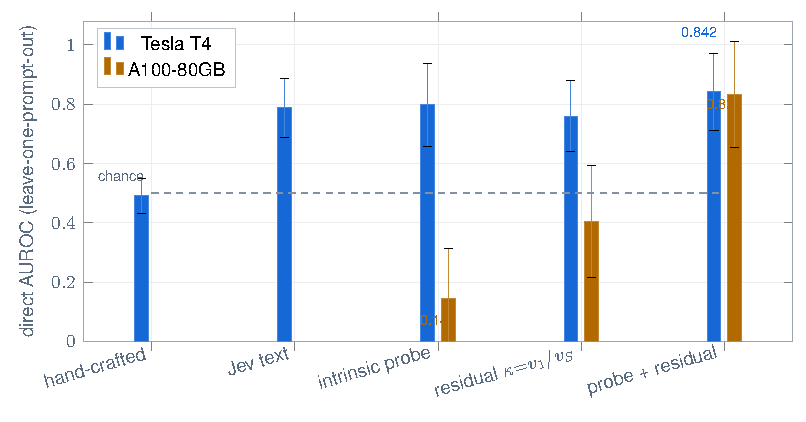
\includegraphics[width=\columnwidth]{figures/fig_signal.pdf}
  \caption{Signal study. On T4 the intrinsic probe (0.798) and the convergence residual (0.752) both beat
  the hand-crafted context statistics (0.491); their combination reaches 0.842. On A100 the intrinsic
  probe \emph{inverts} (0.143) and the residual is at chance (0.485): signals are regime properties.}
  \label{fig:signal}
\end{figure}

\subsection{Seam repair}
Table~\ref{tab:seam} reports the repair sweep. A 25\% blend reduces the boundary seam by 25\% and
\emph{improves} latent fidelity; a hard anchor removes the seam entirely but costs fidelity. The
independent flicker endpoint, however, rises slightly under the repair, so the repair trades a boundary
discontinuity for a small interior flicker. We report the trade rather than a single metric.

\begin{table}[t]
  \centering
  \caption{Seam repair (T4, 32 matched segments). Lower seam and lower fidelity are better. The repair
  reduces the seam and improves fidelity, but the independent flicker endpoint rises.}
  \label{tab:seam}
  \begin{tabular}{lccc}
    \toprule
    variant & boundary seam & fidelity & temporal flicker \\
    \midrule
    none          & 0.614 & 0.761 & 0.0213 \\
    blend 0.25    & \textbf{0.460} & \textbf{0.754} & 0.0218 \\
    blend 0.50    & 0.307 & 0.759 & -- \\
    blend 0.75    & 0.153 & 0.774 & -- \\
    anchor        & 0.000 & 0.799 & -- \\
    fine (no switch) & 0.215 & 0.807 & 0.0254 \\
    \bottomrule
  \end{tabular}
\end{table}

\subsection{Drift propagates on one GPU and reverses on the other}
Figure~\ref{fig:drift} shows drift trajectories for three chains: all-fine, all-coarse, and one coarse
segment followed by fine. On T4 the one-coarse chain remains above the all-fine chain for the rest of the
rollout, and the elevation is significant at four of five tail segments ($+0.021$ to $+0.031$); coarse
error therefore \emph{propagates}. On A100 the coarse chain falls \emph{below} the fine chain: the
comparison reverses. Drift is approximately linear in the segment index, and a transition model fitted on
$(d_t, \text{mode}, t)$ predicts the next drift level at $R^2 \approx 0.94$ only because drift is smooth;
the granularity choice adds nothing ($R^2 \approx 0.01$ for the increment), so a lookahead controller has
little headroom.

\begin{figure}[t]
  \centering
  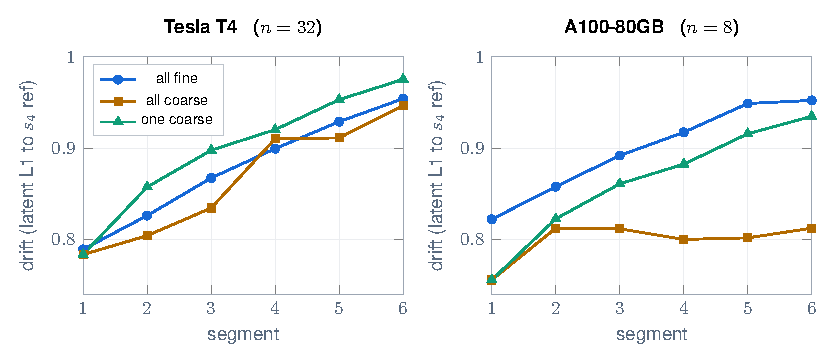
\includegraphics[width=\columnwidth]{figures/fig_drift.pdf}
  \caption{Drift accumulation. On T4 a single coarse segment leaves a persistent elevation (propagation);
  on A100 the coarse chain lies below the fine chain (reversal). Drift is linear and not
  policy-predictable.}
  \label{fig:drift}
\end{figure}

\subsection{The regime map is empty: adaptivity does not pay here}
Table~\ref{tab:policies} reports the policies. On T4 with the two-step pair, fixed fine is both cheaper
and better. On A100, and on T4 with a one-step coarse schedule, fixed coarse is both cheaper and closer to
the reference. In all three cases the adaptive region of Eq.~\eqref{eq:regime} is empty, so the optimal
policy is a fixed mode. This is the paper's central finding, and it is a \emph{design rule}: a practitioner
computes $r$ and $\Delta$ once and deploys accordingly.

\begin{table}[t]
  \centering
  \caption{Policies per operating point. ``Quality'' is the mean endpoint distance (lower is better);
  ``DiT'' is total sampling seconds over the prompt set.}
  \label{tab:policies}
  \begin{tabular}{llccc}
    \toprule
    GPU & policy & DiT (s) & quality & verdict \\
    \midrule
    T4, $s_2/s_2$  & fixed fine   & 281.2 & 0.807 & \textbf{dominant} \\
                   & fixed coarse & 289.6 & 0.752 & dearer \\
    T4, $s_2/s_1$  & fixed fine   & 299.9 & 0.806 & -- \\
                   & fixed coarse & \textbf{218.3} & \textbf{0.755} & \textbf{dominant} \\
    A100, $s_2/s_2$& fixed fine   & 81.9  & 0.780 & -- \\
                   & fixed coarse & \textbf{43.9} & \textbf{0.721} & \textbf{dominant} \\
    \bottomrule
  \end{tabular}
\end{table}

\subsection{Qualitative behaviour}
Figure~\ref{fig:qual} shows matched fine, coarse and repaired segments with an amplified difference map.
The modes produce visibly \emph{different} content --- for the bird prompt the wing pose differs
substantially --- yet no endpoint ranks the coarse mode worse. This is the qualitative counterpart of the
regime map: the modes differ, but neither dominates on quality.

\begin{figure*}[t]
  \centering
  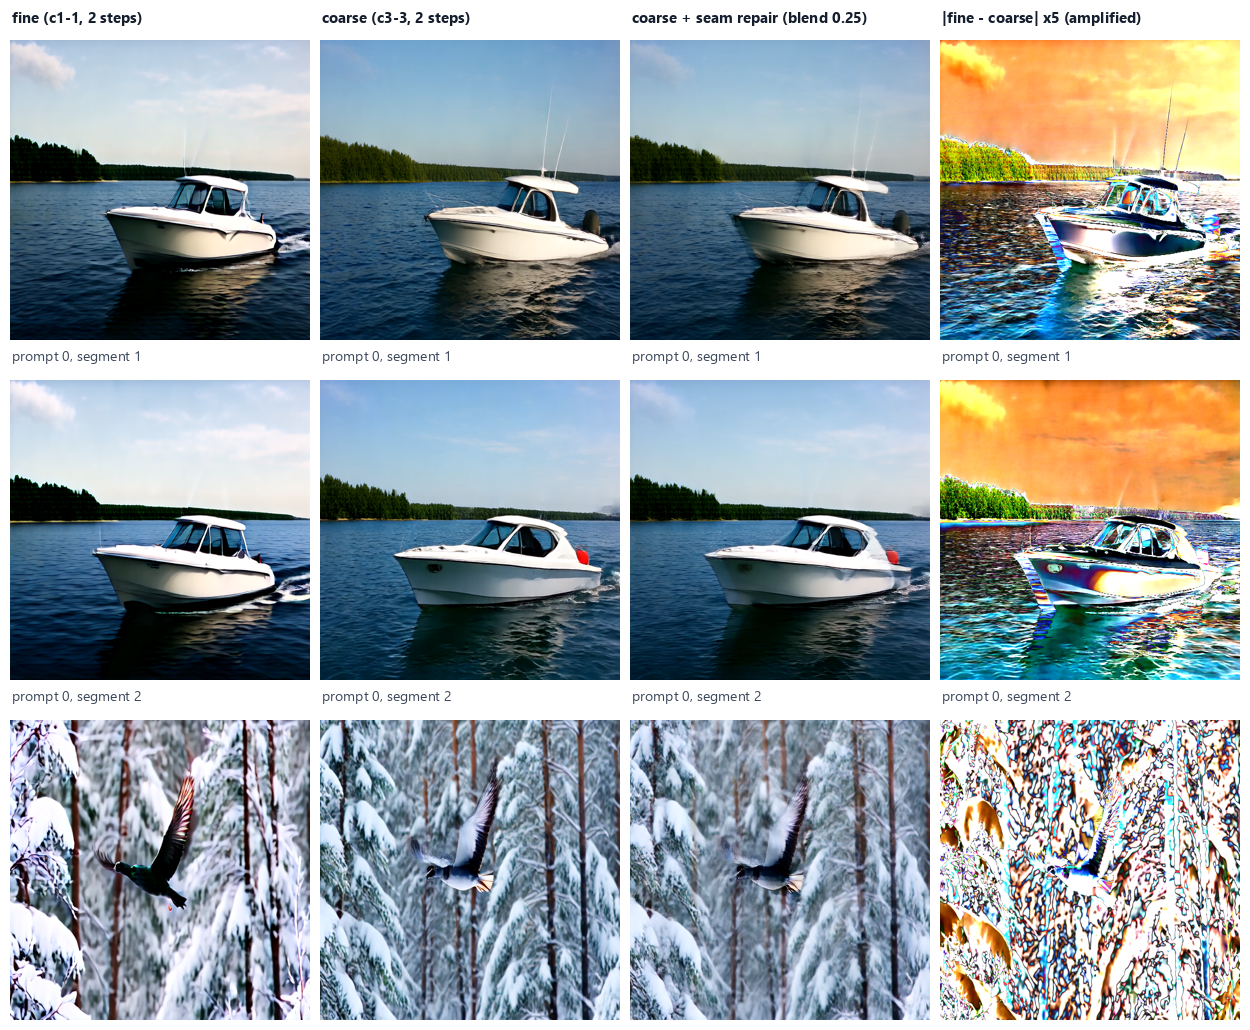
\includegraphics[width=\textwidth]{figures/fig_qualitative.png}
  \caption{Matched segments from the same boundary and noise. Columns: fine, coarse, coarse with the
  25\% seam repair, and the amplified absolute difference between fine and coarse. The modes differ in
  content, yet no independent endpoint ranks coarse as worse.}
  \label{fig:qual}
\end{figure*}

%% ===========================================================================
\section{Boundaries and guidance}
\label{sec:boundaries}

Table~\ref{tab:boundary} lists the boundaries this study establishes, each with its resolution or its
status. We treat a boundary as a result: it delimits the region in which a formulation is valid.

\begin{table}[t]
  \centering
  \caption{Boundary ledger. Each entry is a measured limit of a naive formulation, with its resolution or
  status.}
  \label{tab:boundary}
  \begin{tabular}{p{0.42\columnwidth}p{0.42\columnwidth}c}
    \toprule
    boundary (measured) & resolution & status \\
    \midrule
    cheap context statistics do not predict hard segments (0.491) & intrinsic prefill probe (0.798) & resolved \\
    switching costs a boundary discontinuity & training-free repair ($-25\%$) & resolved \\
    coarse error propagates on T4 & quantified: linear, not compounding & characterised \\
    signals do not transfer across GPUs (0.798 $\rightarrow$ 0.143) & signals are regime properties & open \\
    a context-free critic is at chance (0.497) & critics need context, not pixels & open \\
    the repair raises interior flicker & multi-endpoint protocol required & open \\
    \bottomrule
  \end{tabular}
\end{table}

\paragraph{A practitioner recipe.}
(1) Measure $r$ and $\Delta$ on the target accelerator and schedule. (2) If $r>1$ use fine; if $r<1$ and
$\Delta\le 0$ use coarse; only in the remaining region deploy a router. (3) If a router is deployed,
prefer an intrinsic probe, calibrate its threshold on the target GPU, and never certify the result with
the endpoint used to fit it.

%% ===========================================================================
\section{Conclusion}
\label{sec:conclusion}

Adaptive temporal granularity for causal video world models is not a universal win; it is a decision that
depends on the accelerator, the schedule and the endpoint. We measured the three preconditions on two
GPUs, built an intrinsic signal that needs no external oracle, repaired the switch seam without training,
and derived a regime map that states exactly when a router is worth deploying. At every operating point we
measured, the cheap mode was cheaper and no worse, so a fixed policy is optimal and the adaptive region is
empty. We regard the boundary analysis --- the non-transfer of signals, the linearity of drift, and the
context requirement of decision-model critics --- as the paper's most reusable output, because each
boundary is a design constraint that can be checked before deployment.

%% ===========================================================================
\section*{Declaration of competing interest}
The author declares that he has no known competing financial interests or personal relationships that
could have appeared to influence the work reported in this paper.

\section*{Funding}
This research received no external funding.

\section*{Data availability}
All code, figures and audited result files are publicly available at
\url{https://github.com/j1s4nn/JevGAG}, and the consolidated result bundles are published as public
datasets on Kaggle.

\section*{CRediT authorship contribution statement}
\textbf{Hossen Md Jisan}: Conceptualization, Methodology, Software, Validation, Formal analysis,
Investigation, Data curation, Visualization, Writing -- original draft, Writing -- review and editing.

\section*{Biography}
\begin{wrapfigure}{l}{0.16\textwidth}
  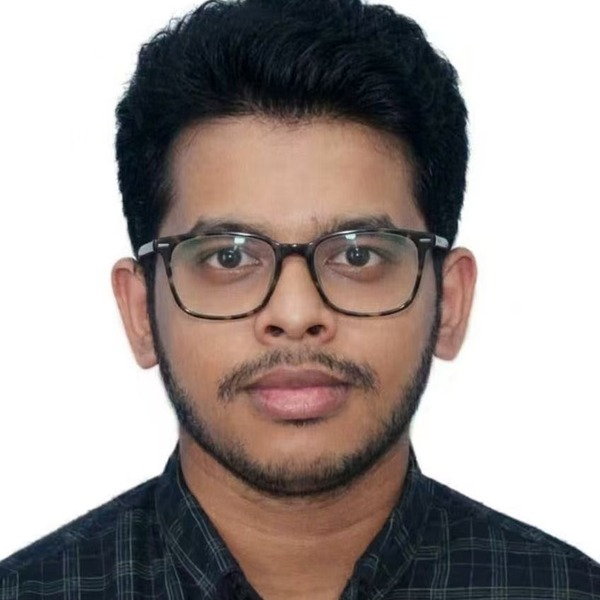
\includegraphics[width=0.15\textwidth]{figures/photo.jpg}
\end{wrapfigure}
\textbf{Hossen Md Jisan} is an undergraduate student of Artificial Intelligence at Nanjing University of
Information Science and Technology (NUIST), Nanjing, China, where he started in September 2023 and is
expected to graduate in June 2027. His research interest is machine vision for embodied intelligence. He
is the author of the prior study on Jev-routed temporal granularity for causal video generation.

\bibliographystyle{cas-model2-names}
\bibliography{refs}

\end{document}
